%----------------------------------------------------------------------------------------
%	SECTION 4
%----------------------------------------------------------------------------------------

\section{Economic, Legal, Social, Ethical and Environmental Context (EL)}

\emph{I cannot submit this section until it has been approved by Sunamp.}




% UNCOMMENT BELOW AFTER SUNAMP FEEDBACK

\begin{comment}

\subsection*{EL1(-, m)}

I gained an understanding of the need for a high level of professional and ethical conduct in engineering and a knowledge of professional codes of conduct in \textit{Procurement and Contracts}.
I familiarised myself with CIBSE's and \hl{...} professional codes of conduct in an assignment where \hl{...}
This course and my ethical induction at Arup also taught me how ethical dilemmas can arise.
\hl{Elaborate?}





\subsection*{EL2}

\begin{wraptable}{r}{0.2\textwidth}
	\begin{tabular}{|ll|}
		\hline
		\multicolumn{2}{|c|}{\cellcolor[HTML]{F8A102}\textbf{EL2}} \\ \hline
		\ID & \DI \\
		\DST & \SIB \\
		Sunamp &  \\ \hline
	\end{tabular}
\end{wraptable}


I have gained knowledge and understanding of the commercial, economic and social context of engineering processes.
A pertinent example which touches all of these aspects is one that I gave in a debate in \IDTitle \space after having heard about it from Stuart MacPherson, the owner of Irons Foulner Consulting Engineers.
Around 2002, Stuart had been appointed to design or refurbish the building services of the Queen's Gallery in Edinburgh (see Figure~\ref{fig:qg}).
Rather than taking the most energy efficient and sustainable approach to the design, he had to consider the social and commercial context of the gallery.
One of the requirements was that none of the services could be visible, as this would not look attractive to the visitors.
Another requirement was that the temperature and humidity levels needed to be maintained within strict ranges so that the artwork would not get damaged.
This is challenging considering that flows of people would be coming in and out of the gallery, possibly with their wet coats and umbrellas on rainy days, causing heat and humidity to constantly be exchanged with the outdoors and the visitors themselves.
In order to isolate the artwork from its environment, so to speak (see Figure~\ref{fig:isolation}), Stuart had to have sensors installed that would detect fluctuations in temperature and humidity, as well as precise ventilation and heating systems that would constantly maintain the acceptable ranges.
This would consequently make the project more expensive, but it was considered necessary for the running of the gallery.

\begin{figure}[htbp]
	\centering
	\begin{subfigure}[b]{0.5\textwidth}
		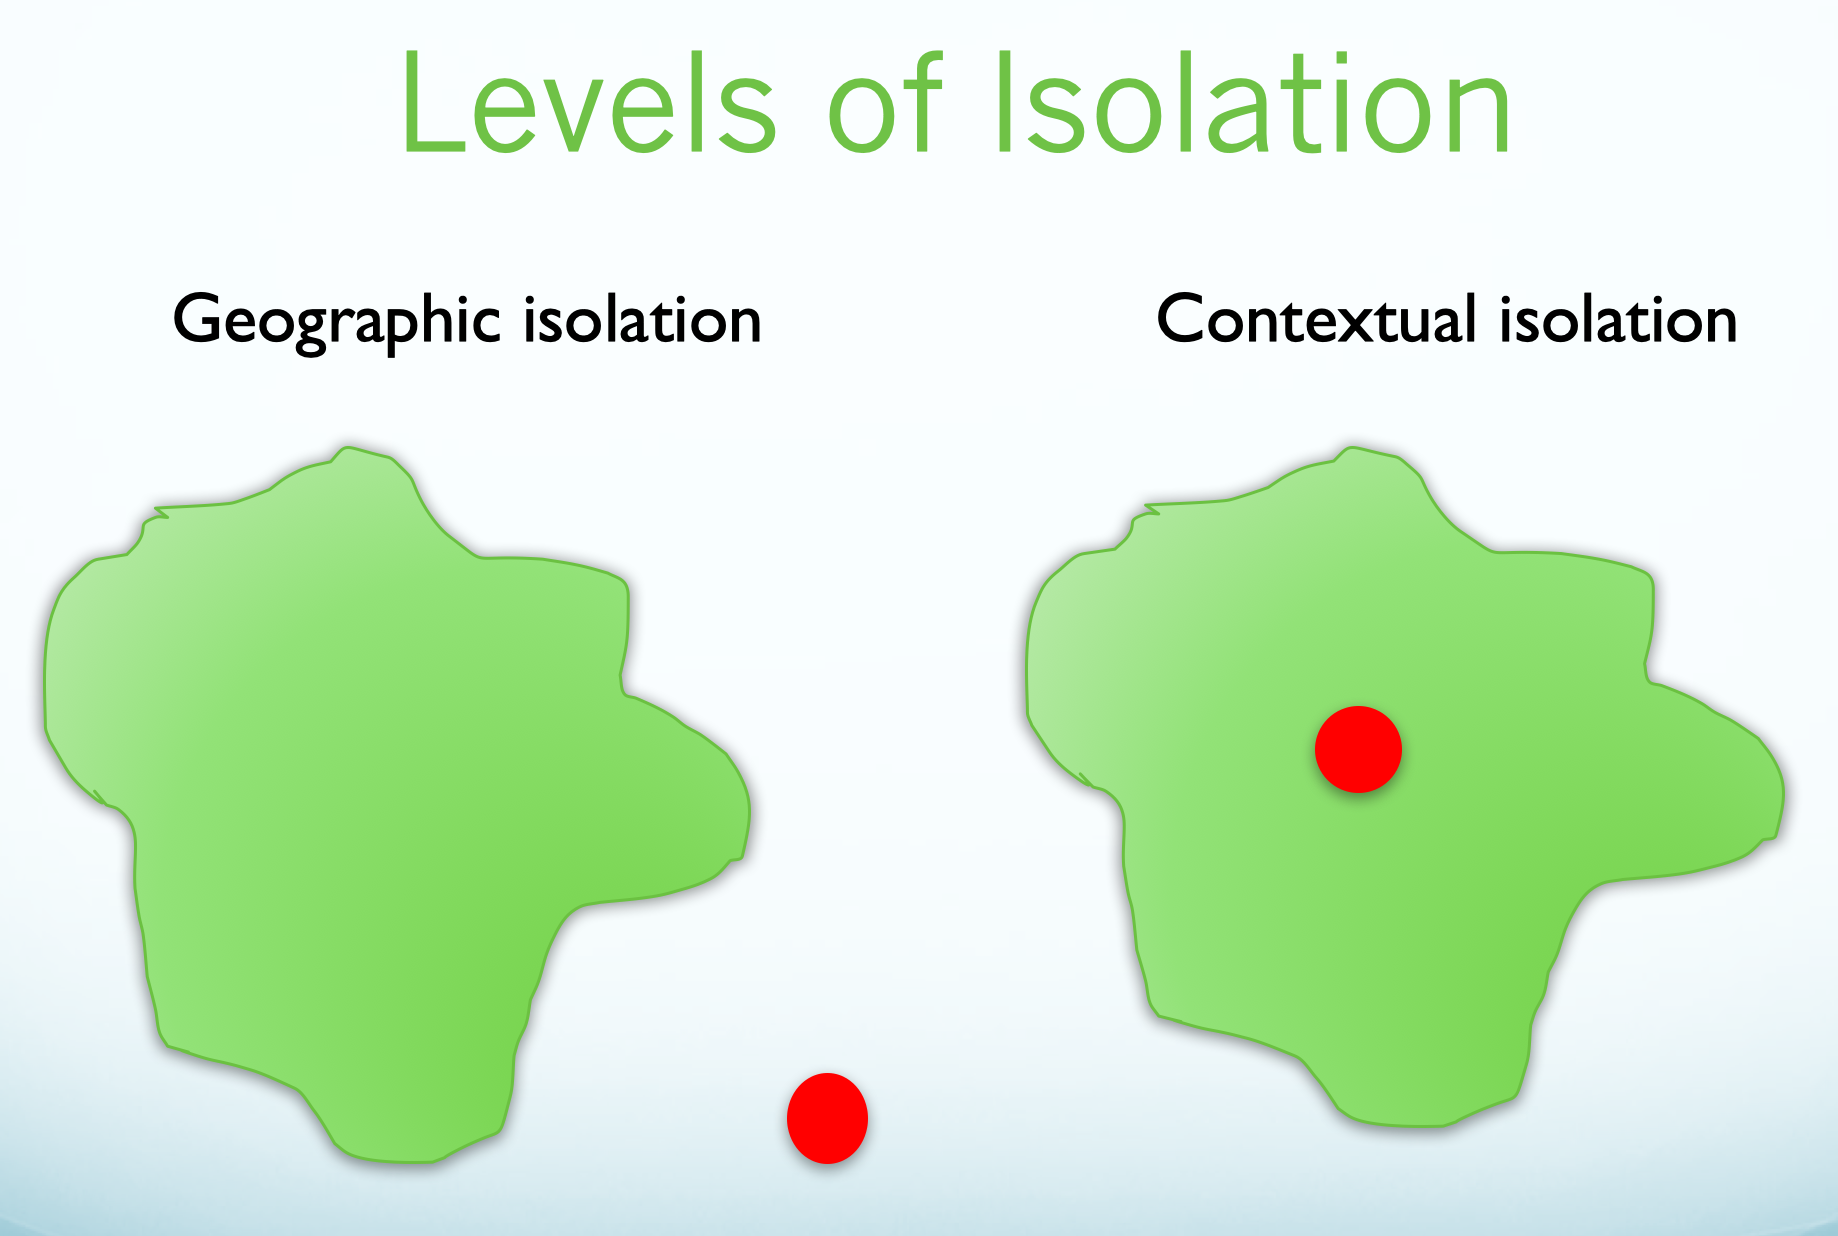
\includegraphics[width=\textwidth]{figures/isolation.png}
		\caption[Contextual isolation.]{A graphical representation of contextual isolation that I created and used in a PowerPoint for a group debate in \ID}\label{fig:isolation}
	\end{subfigure}
	
	\begin{subfigure}[b]{.48\textwidth}
		\centering
		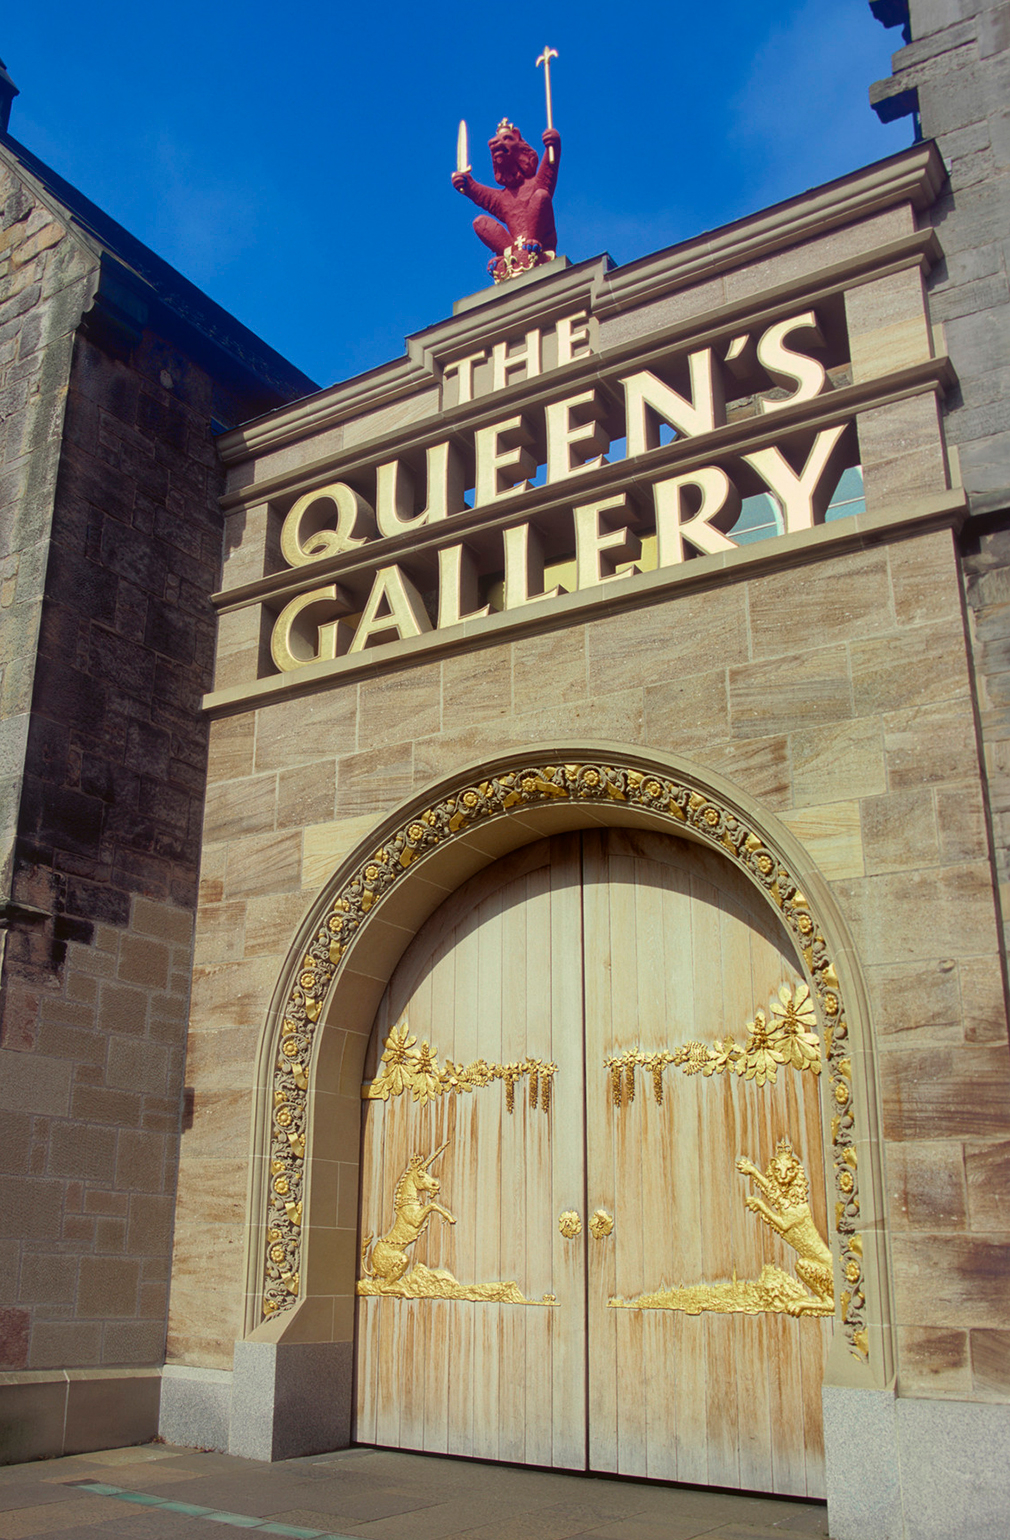
\includegraphics[height=5cm]{figures/gallery-exterior.jpg}
		\caption{Entrance \citep{AboutTheQueensGallery}}\label{fig:qgexterior}
	\end{subfigure}
	\begin{subfigure}[b]{.48\textwidth}
		\centering
		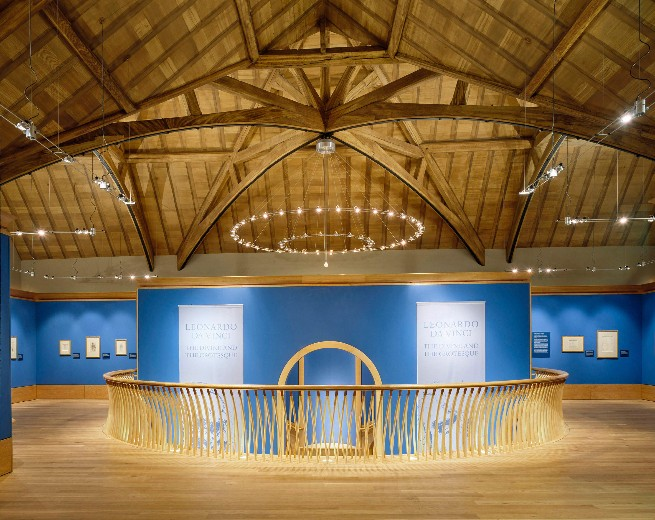
\includegraphics[height=5cm]{figures/gallery-interior.jpg}
		\caption{Interior \citep{InsideTheGallery}}\label{fig:qginterior}
	\end{subfigure}
	\rule{\textwidth}{0.5pt} % use line???
	\caption[The Queen's Gallery and the concept of contextual isolation.]{The Queen's Gallery and the concept of contextual isolation in the design of its building services}
	\label{fig:qg}
\end{figure}





\subsection*{EL3(i, b, m)}

\begin{wraptable}{r}{0.2\textwidth}
	\begin{tabular}{|ll|}
		\hline
		\multicolumn{2}{|c|}{\cellcolor[HTML]{F8A102}\textbf{EL3(i, b, m)}} \\ \hline
		\DST & \LAB \\
		\ICP &  \\ \hline
	\end{tabular}
\end{wraptable}

I gained knowledge of some nascent management techniques that may be used to achieve engineering objectives.
In \ICPTitle, I learned about techniques such as lean construction and supply-chain management (which both have the aim of helping identify flows and wastes) as well as partnering and BIM (which both encourage openness and transparency).

Take lean construction, which is a concept borrowed and adapted from lean manufacturing.
This production method was invented by the Japanese company Toyota shortly after the Second World War.
Japan at the time found itself especially limited in resources due to trade embargoes or restrictions with the Western powers.
Toyota thus had to find a way to make the most use of its restricted resources in order to achieve its production objectives.
Hence, lean manufacturing and construction are about achieving engineering objectives in the most efficient way, i.e. by minimising waste and maximising value.
There are several planning systems that complement this management technique, for example Last Planner which is designed to produce predictable workflows (see Figure~\ref{fig:lastplanner}).


\begin{figure}[htbp]
	\centering
	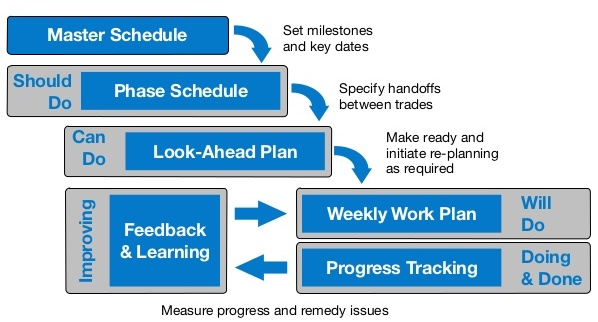
\includegraphics[width=10cm]{figures/last-planner.jpg}
	\rule{10cm}{0.5pt} % use line???
	\caption{The Last Planner system \citep{last-planner}.}
	\label{fig:lastplanner}
\end{figure}


I have some understanding of management techniques since I have used Gantt-like charts on a couple occasions (see Figures~\ref{fig:lab-gantt} and~\ref{DST_schedule}).
When I used the chart to plan the execution of a \LABTitle \space acoustics experiment, it was not very successful.
The chart attempted to coordinate the overlapping activities of our group (which consisted of seven members) within a time limit of 40 minutes so that we could carry out trials on three groups of research participants.
In the end, our experiment ran over time due to our poor timing/ coordination.
The use of the chart was not successful because it was very detailed (on a minute-by-minute basis) and yet we had not familiarised ourselves with it well enough beforehand.
If we were well-rehearsed in the experimental procedure, the use of the Gantt chart could have been more successful.
Hence I learned that there is an element of practice that needs to complement management techniques in order for them to work or run smoothly.

I have not come across change management and do not have enough of experience with management techniques to know their limitations and how they may be applied appropriately.
%Judging from the titles of the upcoming courses of Semester 2, Year 5 (see Table~\ref{tbl:courses}), I suspect I might achieve LO EL3m.
%Considering that this LO should be gained at a Masters level, maybe t
Considering that LO EL3m should be gained at a Masters level, I might learn these things in the second semester of Year 5.
However, judging from the titles of the upcoming courses (see Table~\ref{tbl:courses}), this to me sounds unlikely.





\subsection*{EL4(i, -)}

\begin{wraptable}{r}{0.2\textwidth}
	\begin{tabular}{|ll|}
		\hline
		\multicolumn{2}{|c|}{\cellcolor[HTML]{F8A102}\textbf{EL4(i, -)}} \\ \hline
		\IE & \DPA \\
		\CAS & \EnBldgs \\
		\DI & \FMP \\
		\SIB & \CCSA \\
		\WSD &  \\
		Arup & Hoare Lea \\
		Sunamp & Sweco \\ \hline
	\end{tabular}
\end{wraptable}

I have a good understanding of the requirement for AE activities to promote sustainable development as many of the AE courses have addressed the increasing need for sustainable design to mitigate and adapt to climate change.
%According to the oft-quoted Brundtland report, sustainable development is an approach to progress which meets the needs of the present generation without compromising the ability of future generations to meet their own needs.
%In the context of the built environment, this can be translated as, ``Designing, constructing and managing buildings and resources in such a way that building occupants’ needs are met without the profligate use of energy and resources, such that sufficient provision is left for future generations to provide for themselves" \citep{CCSAunit1}.
%Perhaps because of the direct influence AE has on particularly the energy consumption of a building, many of the courses throughout the programme have addressed the increasing need for sustainable design to mitigate and adapt to climate change.
I especially realised the importance of this engineering requirement as I came across a response CIBSE offered in a governmental consultation during my research for a group poster for \CCSATitle.
%(see description of assignment in \textit{G1} in Section \ref{sec:G1}), 
%At the start of 2018,
Before the publication of the 2018 National Adaptation Programme (NAP) to climate change, 
the government suggested that adaptation reporting continues to be done on a voluntary basis.
However, CIBSE protested by stressing that adaptation is necessary because climate change threats are real and imminent, so reporting should be done on a mandatory basis by even more sectors than have been required of so far \citep{CIBSE:CCAreporting}.
Unfortunately, according to the 2018 NAP, the government will not make reporting mandatory because the majority of the respondents to the consultation favoured the continuation of voluntary reporting \hl{cite NAP from Mendeley}.
Perhaps if more engineering institutions acted like CIBSE and promoted the urgency of sustainable development in this consultation, as is their duty, the government's stance on sustainable development might have been stronger.

\begin{wrapfigure}{r}{0.5\textwidth}
	\centering
	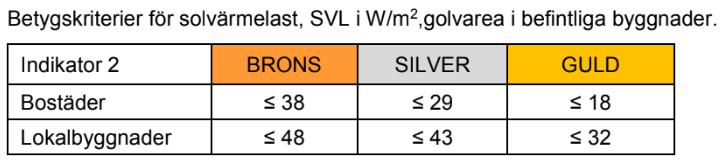
\includegraphics[width=0.5\textwidth]{figures/SVL.PNG}
	\rule{0.5\textwidth}{0.5pt} % use line???
	\caption[The \textit{Miljöbyggnad} assessment criteria for solar heat gains in existing buildings.]{The \textit{Miljöbyggnad} assessment criteria for solar heat gains (in W/m\textsuperscript{2}) in existing buildings \hl{cite miljobyggnad}.}
	\label{fig:svl}
\end{wrapfigure}

I also have the ability to apply quantitative techniques to promote sustainable development.
An example is the work I did at Sweco on environmental certification, a way to promote the sustainable design of buildings.
I calculated and ranked things like solar heat gains, energy consumption and daylighting according to \textit{Miljöbyggnad}'s standards of what qualified as a sustainable building (see Figure~\ref{fig:svl}).


%According to the oft-quoted Brundtland report, sustainable development is an approach to progress which meets the needs of the present generation without compromising the ability of future generations to meet their own needs.
%\hl{Can't think of examples. Also, ability to apply quantitative techniques???}



\subsection*{EL5(-, m)}

The following courses increased my awareness of legal requirements governing engineering activities including \hl{health and safety (H\&S)}, liability issues, contracts and accessibility:
\textit{Design Issues},
\textit{Procurement and Contracts},
and \textit{Inclusive and Safe Environments}.
In particular, in \textit{Design Issues} I learned about the various UK regulations surrounding H\&S, including the Health and Safety at Work Act 1974 and the Construction (Design and Management) Regulations 2015, a.k.a. the CDM Regulations.
The CDM Regulations emphasise that H\&S need to be considered, not just on site, but throughout the planning and design stages also.
The designers, for example, have a responsibility to assess and eliminate or mitigate the H\&S risks associated with their design, whether that is during the construction or operation of the building.
Furthermore, this course broadened my awareness of legal requirements outside of the UK.
I learned about the H\&S regulations in France, the lack of building regulations in Guyana, and the ambitious building regulations with regards to sustainability in Singapore.
\hl{Is that a good demonstration of my knowledge? David: provide two references.}

I have also applied my knowledge of legal requirements in a project for \textit{Inclusive and Safe Environments} and during my placements at Hoare Lea and Sweco.
At Hoare Lea I produced \hl{RIBA} Stage 3 layouts of fire detection and alarm installations for a new-build.
These were made to comply with standards such as \textit{BS 5839-6:2013 Fire detection and fire alarm systems for buildings - Part 6: Code of practice for the design, installation, commissioning and maintenance of fire detection and fire alarm systems in domestic premises}.
For instance, the standard stated the different radiuses that smoke detectors and heat detectors cover; I had to thus place the detectors on the plan layouts accordingly.


\subsection*{EL6(i, b, m)}

Many courses and a couple of my placements increased my awareness of risk issues.
I learned about risk issues related to H\&S at Sunamp and in
\textit{Electrical and Lighting Services for Buildings},
\textit{Design Issues},
\textit{Inclusive and Safe Environments},
and
\textit{Laboratory Project}.
In \textit{Electrical and Lighting Services for Buildings}, for example, I learned about the importance of earthing to give \hl{overflow?} electricity an alternative path to run through which is not a person (thus electrocuting them).
I learned about environmental risk issues in
\textit{Construction Technology 1},
\textit{Introduction to the Environment},
\textit{Thermal Performance Studies},
\textit{Sustainable and Intelligent Buildings},
\textit{Climate Change, Sustainability and Adaptation},
and
\textit{Water Supply and Drainage for Buildings}.
Throughout these courses I have learned about the impact of buildings and building systems on the environment, e.g. harmful refrigerants in air conditioners, embodied carbon in building materials, and the emissions from vehicles that people use to travel to buildings.
Lastly, I learned about \hl{commercial risk (?)} in \textit{Innovation in Construction Practice}, more specifically the risk of innovation in construction projects.
\hl{Elaborate?}

I learned about the techniques of risk assessment and risk management in depth in \textit{Design Issues} and have carried out H\&S risk assessments in \textit{Facilities Management Principles}, \textit{Laboratory Project} and during my placement at Arup.
\hl{Attach LAB risk assessments?}
Generally, one first needs to identify the risks and then assess them in terms of severity and likelihood.
Afterwards, one tries to eliminate the risks (the worst first), and if that is not possible, mitigate them.


\subsection*{EL7m}

For business success, I have only gained an understanding of how innovation is a key driver in \textit{Innovation in Construction Practice} and \hl{how technology (?) plays a role in business success through the study of Fordist and post-Fordist consumerism/ manufacturing?} in \textit{Sustainable and Intelligent Buildings}.
\hl{Look up ICP and SIB notes + elaborate.}

Due to the nature of my academic programme, I have not learned as much about the key drivers for business success as I have for successful construction projects in the following courses:
\textit{Introduction to Design},
\textit{Procurement and Contracts},
\textit{Facilities Management Principles},
\hl{and more?}
However, there are two ways that this knowledge can translate to business.
Firstly, a construction project is often a means for a business to grow or improve (\hl{this is known as a secondary business case? see FM notes}).
Therefore, a successful construction project can lead to a successful business.
Secondly, the principles behind a successful construction project should also be able to be applied to businesses.
For example, after the construction sector was pointed out in the 1990s for repeatedly delivering projects that were of poor quality, overtime and over-budget, the sector has made significant efforts to improve its performance and improve client satisfaction.
Such efforts have resulted in changing the workflow so that more planning is done at the start of a project, when making changes is more flexible and less costly (\hl{get figure from ICP?}).
This includes developing more descriptive briefs, which set out the client's needs and how the construction project should be run.
\hl{I imagine this could translate in such a way to business... think!}


\end{comment}